%%=============================================================================
%% Proof of concept
%%=============================================================================

\chapter{Proof of Concept}%
\label{ch:proofofconcept}

\section{Dataset} \label{sec:poc-dataset}
Uit de voorgaande literatuurstudie in hoofdstuk ~\ref{sec:dataset} kan geconcludeerd worden dat de FairFace dataset van \textcite{Karkkainen2021} de meest geschikte is voor gezichtsanalyse. Deze dataset wordt beschikbaar gesteld via Google Drive of Kaggle. De dataset is beschikbaar met een padding (marge) van 0.25 of 1.25. Voor deze Proof of Concept wordt de dataset met een padding van 0.25 gebruikt. Deze is het meest geschikt voor wetenschappelijk onderzoek, omdat deze door de kleinere marge minder opslag verbruikt en het volledige gezicht weergeeft. De dataset is verder opgedeeld in 86.744 train afbeeldingen en 10.954 validatie of test afbeeldingen. Dit maakt de FairFace dataset een bijzonder grote dataset met kleine bias en beperkte opslag, wat ideaal is voor wetenschappelijk onderzoek. \\
\\
Doordat de zip folder te groot is om direct te downloaden en steeds een waarschuwing genereert via Google Drive, moet de dataset gedownload en uitgepakt worden. Dit kan manueel, of efficiënter in Python via codevoorbeeld ~\ref{sc:dataset} . De dataset kan dus niet in memory opgeslagen worden of rechtstreeks in Google Drive worden aangesproken.\\
\\
De labels van de trainingsset bevinden zich in een csv bestand (in dezelfde Google Drive). Om uit te testen of de dataset correct werd ingeladen, is het mogelijk om enkele willekeurige afbeeldingen weer te geven met hun leeftijdscategorie en geslacht label. In deze Proof of Concept wordt dan ook een leeftijdscategorie voorspelt en geen leeftijdsgetal. Dit zorgt ervoor dat het voorspellen van de leeftijd een classificatietaak wordt, net zoals het voorspellen van geslacht. Wanneer er een leeftijdsgetal wordt voorspeld, is dit een regressieprobleem \autocite{Geron2019}. Een voorbeeld van de uitvoer van deze test wordt weergegeven op figuur~\ref{fig:5randomtrain}. Voor deze Proof of Concept worden enkel de labels voor de leeftijd en geslacht gebruikt. Daarnaast bevat de FairFace dataset ook een label voor ras.

\begin{lstlisting}[style=mystyle, caption={Functie om FairFace dataset te downloaden en uitpakken \autocite{Ramos2024}}, label={sc:dataset}]
# Download the dataset from Google Drive and save in the data directory
# URL to the Google Drive file
url = 'https://drive.google.com/u/0/uc?id=1Z1RqRo0_JiavaZw2yzZG6WETdZQ8qX86&export=download'

zip_file = gdown.download(url, quiet=False)

destination_dir = './data'
os.makedirs(destination_dir, exist_ok=True) # Create the directory if it doesn't exist

# Extract the zip file into the specified directory
with zipfile.ZipFile(zip_file, 'r') as z:
z.extractall(destination_dir)
\end{lstlisting}



\begin{figure}
    \centering
    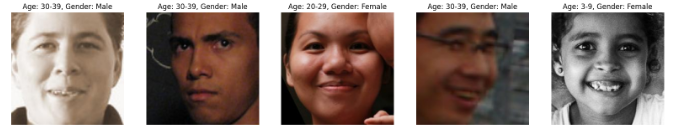
\includegraphics[width=\columnwidth]{graphics/randomtrain.png}
    \caption[5 willekeurige train voorbeelden]{5 willekeurige train voorbeelden met leeftijd en geslacht label}
        \label{fig:5randomtrain}}
\end{figure}

\section{Feature extractie} \label{sec:poc-featextractie}
De feature extractie is de eerste preprocessing stap in de machine learning pipeline. In deze Proof of Concept wordt het getrainde dlib model van \textcite{King2024} gebruikt. Dit model detecteert en voorspelt de 68 landmarks uit het gezicht. Het model is beschikbaar via GitHub en is beperkt in opslag. Doordat het model al voorgetraind is, hoeft dit dus niet opnieuw getraind te worden en versnelt het preprocessing proces. Door het detecteren van de landmarks kunnen we deze behouden en de afbeelding normaliseren, zoals in {~\ref{sub:normalisatie}}. \\
\\
\textcite{King2024} stelt ook een model ter beschikking waarop slechts 5 landmarks gedetecteerd worden. Dit zijn de 2 uiteinden van de ogen en het midden van de neus. Figuur ~\ref{fig:5landmarks} geeft een voorbeeld van een gezichtsafbeelding waarop deze 5 landmarks worden aangeduid. Voor deze use case zijn de 5 landmarks duidelijk te weinig om de volledige vorm van het gezicht weer te geven. Dit model met 5 landmarks is efficiënter bij een simpele gezichtsdetectie, om opslag te besparen en het model te versnellen.

\begin{figure}[H]
    \centering
    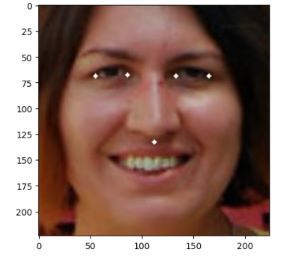
\includegraphics[width=\columnwidth]{graphics/5landmarks.PNG}
    \caption[5 landmarks op het gezicht]{5 landmarks op het gezicht}
    \label{fig:5landmarks}}
\end{figure}

\begin{enumerate}
    \item De eerste stap in dit proces omvat het detecteren van de 68 landmarks  \autocite{Serengil2020}. Deze omvatten de vorm van het gezicht, wenkbrauwen, ogen, neus en mond. Dit wordt uitgevoerd met het \textit{shape\_predictor\_68\_face\_landmarks} model van \textcite{King2024}. Vervolgens wordt de \textit{circle} functie van \textcite{OpenCV2024} gebruikt om de landmarks aan te duiden op de afbeelding. \\
    Figuur {~\ref{fig:68landmarks} geeft het resultaat van deze stap weer. \\
    \item Vervolgens wordt op basis van de gedetecteerde landmarks de vorm van het gezicht uit de afbeelding gehaald. De coördinaten van deze landmarks worden opgehaald en met \textit{line} van \textcite{OpenCV2024} omcirkeld. Er wordt een lijn getrokken van het eerste punt naar het volgende in de lijst met coördinaten. Figuur {~\ref{fig:gezichtsvorm}} geeft het resultaat van deze stap. \\ 
    \item Ten slotte maken we een mask voor de overgebleven afbeelding. Alles rond de vorm van het gezicht wordt met \textit{fillConvexPoly} van \textcite{OpenCV2024} zwart ingekleurd. Hierdoor wordt de onbelangrijke achtergrond van de afbeelding verwijdert en wordt enkel het gezicht overgehouden. Deze stap voert de normalisatie net zoals \textcite{Chen2011} uit, gebruikmakend van de HOG features in het detecteren van de landmarks, omschreven in  ~\ref{sub:hog}. Figuur {~\ref{fig:normalisatie}} geeft het resultaat van deze stap weer. Dit is een genormaliseerde afbeelding die gebruikt zal worden voor de feature dimensionaliteitsreductie.
\end{enumerate}\\

Het normaliseren van de afbeeldingen kan in een functie worden gestoken. Hierdoor kan aan de volledige dataset een mask toegevoegd worden, in plaats van slechts 1 afbeelding voordien. Het toevoegen van een mask aan een afbeelding duurt minder dan een seconde. Dit maakt deze methode geschikt voor de grote dataset.  Het toevoegen van de mask wordt in batches gedaan, om het proces te versnellen. Er wordt hierdoor steeds aan een aantal afbeeldingen tegelijk een mask toegevoegd, in plaats van 1 afbeelding per keer. Er wordt gekozen voor een batch size van 128, omdat deze voldoende groot is voor de beschikbare rekenkracht op een standaard laptop. Het volledige proces nam 84 minuten in beslag voor 86.744 afbeeldingen. \\
\\
Daarnaast kan deze functie ook valideren dat er geen duidelijke gezichten aanwezig zijn op de afbeeldingen, doordat de 68 landmarks niet gedetecteerd kunnen worden. Deze afbeeldingen zijn onbruikbaar en worden zo ook uit de dataset gehaald. Figuur {~\ref{fig:noface}} geeft een afbeelding weer waarop de landmarks niet gedetecteerd kunnen worden. Dit komt doordat de foto geen vooraanzicht is en op deze figuur zijn beide ogen niet duidelijk weergegeven.  Codevoorbeeld {~\ref{sc:mask} geeft deze functie weer \autocite{Serengil2020}. In de genormaliseerde trainingsdataset blijven nog 63.938 afbeeldingen over, in de genormaliseerde testset blijven nog 8.028 over. Beide datasets verliezen na normalisatie zo ongeveer 27\% van de gezichtsafbeeldingen, maar zijn nog voldoende groot om mee verder te werken.

\begin{figure}[H]
    \centering
    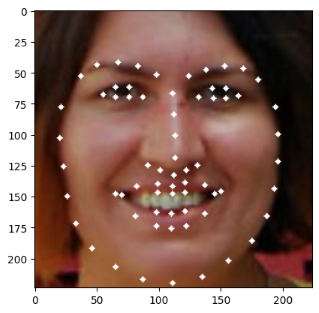
\includegraphics{graphics/68landmarks.png}
    \caption[68 landmarks op gezicht]{68 landmarks op het gezicht}
    \label{fig:68landmarks}}
\end{figure}

\begin{figure}[H]
    \centering
    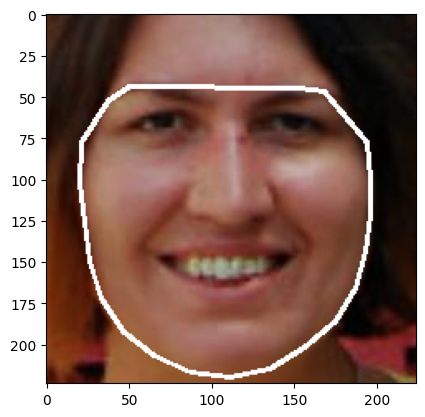
\includegraphics{graphics/gezichtsvorm.png}
    \caption[Gezichtsvorm uit afbeelding halen]{Gezichtsvorm uit afbeelding halen op basis van landmarks}
    \label{fig:gezichtsvorm}}
\end{figure}

\begin{figure}[H]
    \centering
    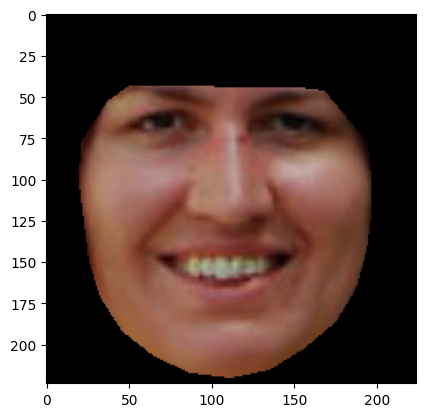
\includegraphics{graphics/normalisatie.png}
    \caption[Normalisatie van gezichtsafbeelding]{Normalisatie van gezichtsafbeelding}
    \label{fig:normalisatie}}
\end{figure}

\begin{lstlisting}[style=mystyle, caption={Functie om mask toe te voegen aan de volledige dataset \autocite{Serengil2020}}, label={sc:mask}]
import os
import cv2
import dlib
import numpy as np

def get_mask(image_paths, predictor_path, output_folder):
# Initialize face detector and landmark detector
face_detector = dlib.get_frontal_face_detector()
landmark_detector = dlib.shape_predictor(predictor_path)

for image_path in image_paths:
image = dlib.load_rgb_image(image_path)

# Detect faces in the image -> do not mask images where no face is found
faces = face_detector(image, 1)
no_faces = []
if len(faces) == 0:
print("No faces found in the image:", image_path)
no_faces.append(image_path)
continue

# Predict facial landmarks
face = faces[0] # only one face
landmarks = landmark_detector(image, face)
landmarks_tuple = [(landmarks.part(i).x, landmarks.part(i).y) for i in range(68)]

# Define the route for the mask
routes = [i for i in range(16,-1,-1)] + [i for i in range(17,19)] + [i for i in range(24,26)] + [16]
routes_coordinates = [landmarks_tuple[i] for i in routes]

# Create a mask
mask = np.zeros((image.shape[0], image.shape[1]), dtype=np.uint8)
mask = cv2.fillConvexPoly(mask, np.array(routes_coordinates), 255)
masked_image = cv2.bitwise_and(image, image, mask=mask)

# Save the masked image to the output folder with the same filename
filename = os.path.splitext(os.path.basename(image_path))[0]
output_filename = filename + "_masked.jpg"
output_path = os.path.join(output_folder, output_filename)
cv2.imwrite(output_path, masked_image)

print("Masked image saved:", output_path)

# Configuration
predictor_path = "./shape_predictor_68_face_landmarks.dat"
input_folder = 'data/train'
output_folder = './data/masked_train'
batch_size = 128

# Create the output folder if it doesn't exist
if not os.path.exists(output_folder):
os.makedirs(output_folder)

# List all image files in the input folder
image_files = sorted([f for f in os.listdir(input_folder) if f.endswith(('.jpg', '.jpeg', '.png'))], key=lambda x: int(os.path.splitext(x)[0]))

# Process images in batches
for i in range(0, len(image_files), batch_size):
batch_images = image_files[i:i+batch_size]
batch_paths = [os.path.join(input_folder, image) for image in batch_images]
get_mask(batch_paths, predictor_path, output_folder) 
\end{lstlisting} 
\begin{figure}
    \centering
    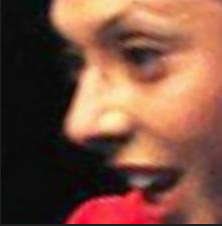
\includegraphics{graphics/no_face_detected.png}
    \caption[Geen gezicht gedecteerd op afbeelding]{De 68 landmarks werden niet teruggevonden op de gezichtsafbeelding, deze wordt verwijderd uit de dataset.}
    \label{fig:noface}}
\end{figure}

% ---- Feature dim
\section{Feature dimensionaliteitsreductie}\label{sec:poc-featuredim}
Op de genormaliseerde afbeeldingen wordt Truncated SVD toegepast als dimensionaliteitsreductie van de features. Doordat de dataset zeer veel afbeeldingen bevat, wordt geopteerd voor Truncated SVD in plaats van het gekende PCA. PCA vereist een enorme rekenkracht op een grote dataset, omdat deze de covariantie van de matrix van de originele dataset berekent. Truncated SVD berekent de singular value decomposition van de datamatrix, wat veel efficiënter is voor grote en sparse datasets \autocite{Baruah2023}. De benodigde opslag zal verminderen en de impact van noise op de dataset daalt. Het uitvoeren van PCA op de dataset, of zelfs een subset daarvan, genereert meteen een foutmelding over de benodigde opslag. Een standaard laptop kan deze berekening niet aan.\\
\\
De Truncated SVD functie wordt beschikbaar gesteld via \textit{sklearn.decomposition}. Aan Truncated SVD wordt het aantal componenten, dat behouden moet worden, als paramater meegegeven. Dit is de gewenste dimensionaliteit van de output data. De dimensionaliteit moet steeds minder zijn dan het aantal features in de data \autocite{ScikitLearn2024}. Het ideale aantal componenten kan berekend worden aan de hand van de verklaarde variantie. Er wordt een lus gemaakt door de Truncated SVD met een range die gaat tot de shape van de trainingsdata. Voor elk aantal componenten wordt de verklaarde variantie berekend. De grafiek met de verklaarde variantie per aantal componenten kan teruggevonden worden op figuur {~\ref{fig:explainedvar}}. \\
\\ 
Er wordt verder gewerkt met 400 componenten, omdat deze een verklaarde variantie van circa 0.99 heeft. Hierdoor daalt het aantal componenten van de data van 1000 naar 400. De features van data worden zo gereduceerd om makkelijker mee verder te werken bij het trainen van de machine learning modellen. Codevoorbeeld {~\ref{sc:truncatedsvd} geeft weer hoe de Truncated SVD wordt toegepast op de volledige trainingsdataset. Het resultaat van de dimensionaliteitsreductie op een gezichtsafbeelding is te vinden op figuur {~\ref{fig:truncated}}.
\begin{figure}[H]
    \centering
    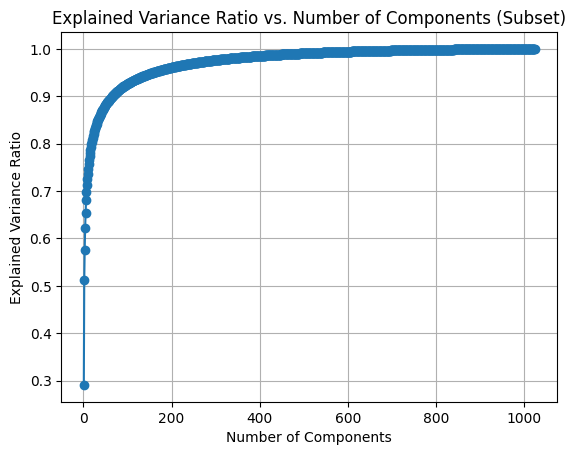
\includegraphics{graphics/explained_variance.png}
    \caption[Verklaarde variantie voor de Truncated SVD]{Verklaarde variantie voor de Truncated SVD}
    \label{fig:explainedvar}}
\end{figure}
\begin{lstlisting}[style=mystyle, caption={Functie om Truncated SVD toe te passen op de volledige dataset \autocite{ScikitLearn2024}}, label={sc:truncatedsvd}]
% Apply TruncatedSVD for dimensionality reduction
svd = TruncatedSVD(n_components=400)
X_train_svd = svd.fit_transform(X_train)  
\end{lstlisting}
\begin{figure}[H]
    \centering
    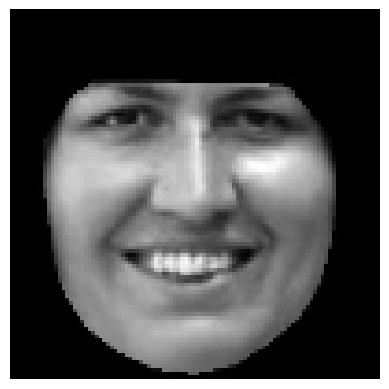
\includegraphics{graphics/truncatedsvd.png}
    \caption[Truncated SVD toegepast op genormaliseerde gezichtsafbeelding]{Truncated SVD toegepast op genormaliseerde gezichtsafbeelding}
    \label{fig:truncated}}
\end{figure}

\section{Machine learning modellen}\label{sec:poc-mlmodellen}
Om het meest geschikte machine learning model te vinden voor de voorspelling van leeftijd en geslacht op basis van gezichtsafbeeldingen, worden verschillende modellen uit de literatuurstudie in hoofdstuk ~\ref{sec:bestaandeml} getest. De performantie van 2 aparte modellen die leeftijd en geslacht voorspellen, alsook 1 model die beide voorspelt worden geanalyseerd. \\
\\
Om optimaal te zoeken naar de beste parameters wordt gebruik gemaakt van GridSearch ~\ref{sub:gridsearch}. Hieraan worden meerdere parameters meegegeven, zoals aantal estimators of kernel, waarvoor GridSearch de parameter met de beste score na training weergeeft. Aan de parameters van Grid Search wordt 5 als standaardwaarde van de cross validatie meegegeven. Zoals in ~\ref{sub:gridsearch} aangehaald, worden er 5 herhalingen uitgevoerd op de dataset om het model te optimaliseren. De modellen met hun parameters worden geëvalueerd op basis van de balanced accuracy. Deze score gaat het aantal correct voorspelde instanties na, in een dataset die mogelijks ongelijk verdeeld is \autocite{Garcia2009}. Tabel ~\ref{tab:leeftijdcat} geeft weer hoe de leeftijdscategorieën verdeeld zijn en tabel ~\ref{tab:geslacht} hoe geslacht verdeeld is in de trainingsdata. Hieruit kan afgeleid worden dat de leeftijdscategorieën niet even verdeeld zijn en dat balanced accuracy hier wel degelijk de betere optie is. \\
\\
De testfase van de GridSearch wordt uitgevoerd op een subset van 1000 willekeurige afbeeldingen uit de dataset om de tijd die nodig is om te trainen te verminderen. Het model met de parameters die de beste score leveren, wordt dan uiteindelijk getraind op de volledige trainingsdataset. \\
\begin{center}
    \caption{Verdeling van leeftijdscategorieën}
    \label{tab:leeftijdcat}
    \begin{tabular}{||c | c | c||} 
        \hline
        Leeftijdscategorie & Aantal & Percentage van volledige dataset  \\ 
        \hline
        0-2 & 1399 & 2,19\% \\
        \hline
        3-9 & 8003 & 12,52\% \\
        \hline
        10-19 & 6880 & 10,76\% \\
        \hline
        20-29 & 18924 & 29,60\% \\
        \hline 
        30 -39 & 13874 & 21,70\% \\
        \hline
        40-49 & 7726 & 12,08\% \\
        \hline 
        50-59 & 4528 & 7,08\% \\
        \hline 
        60-69 & 1980 & 3,10\% \\
        \hline 
        more than 70 & 624 & 1\% \\
    \end{tabular}
\end{center}

\begin{center}
     \caption{Verdeling van geslacht}
       \label{tab:geslacht}
    \begin{tabular}{||c | c | c||} 
        \hline
        Geslacht & Aantal & Percentage van volledige dataset  \\ 
        \hline
        Male & 32435 & 50,73\% \\
        \hline
        Female & 31503 & 49,27\% \\
        
    \end{tabular}
\end{center}

\\
Om een model te trainen die beide (leeftijd en geslacht) gelijktijdig kan voorspellen, wordt gebruik gemaakt van de MultiOutputClassifier van \textit{sklearn.multioutput}. Deze strategie bestaat uit het aanpassen van een classifier per target. Hiermee kunnen classifiers uitgebreid worden die van nature geen multi-target classificatie ondersteunen, zoals Random Forest Classifier \autocite{ScikitLearn2024}. Het model geeft als output 2 labels, één voor geslacht en één voor de leeftijdscategorie. \\
\\ 
Het getrainde model wordt getest op de validatie dataset. Dit gebeurt met de \textit{predict} functie van Scikit-learn. Op basis hiervan wordt de confusion matrix opgesteld en de performantiescores, aangehaald in de literatuurstudie ~\ref{ch:standvanzaken}, berekent. \textcite{ScikitLearn2024} heeft al enkele ingebouwde functies om de performantiescores, zoals $accuracy\_score$ en $precison\_score$, te berekenen. Deze kunnen uitgevoerd worden op de confusion matrix van het geslacht. Voor de modellen die leeftijd en beide voorspellen dienen de scores handmatig berekend te worden, omdat dit geen 2x2 matrices zijn. 

\subsection{Random Forest Classifier} \label{sub:poc-rfc}
Het Random Forest Classifier model wordt beschikbaar gesteld via \textit{sklearn.ensemble}.
Omdat het model geen tekstuele data kan categoriseren, dienen de labels omgezet te worden naar numerische waarden. Voor het geslacht (Female of Male) wordt dit 0 of 1. Voor de leeftijdscategorieën wordt OrdinalEncoder gebruikt om deze te mappen naar een getal tussen 0 en 8, waarbij '0-2' categorie 0 wordt en 'more than 70' categorie 8 wordt. Aan deze Ordinal Encoder geven we een mapping mee van de labels. De encoder gaat deze dan fitten op de gegeven labels van de dataset volgens de meegegeven mapping \autocite{ScikitLearn2024}.  \\
\\
Aan de Grid Search voor de Random Forest Classifier worden volgende parameters meegegeven:
\begin{itemize}
    \item $n\_estimators$: het aantal bomen dat gebruikt wordt (default = 100). 
    \item $max\_features$: het aantal features die gebruikt worden om de beste scheiding in de bomen te vinden (default = 'sqrt')
    \item $min\_samples\_split$: het minimum aantal instanties die nodig zijn om node te mogen splitsen (default = 2).
    \item $min\_samples\_leaf$: minimum aantal instanties die in een blad moeten zitten (default = 1). Een blad is het uiteinde van een boom, die de voorspelde klasse weergeeft \textcite{Garg2020}. 
    \item $max\_depth$: de maximale diepte van een boom (default = None). 
    \item bootstrap: het gebruik van steekproeven bij het bouwen van de bomen (default = True)
\end{itemize}
\\
\begin{center}
    \begin{tabular}{||c | c  | c | c||} 
        \hline
          & Geslacht & Leeftijd & Beide  \\ 
        \hline
        Parameters & $n\_estimators=230$ & $max\_depth$=5, $n\_estimators$=200 & $n\_estimators$=100  \\ 
        \hline
        Accuracy & 99,99\% & 29,71\% & 99,95\%  \\
        \hline
        Precision & 99,99\% & 0,00\% & 99,93\%  \\
        \hline
        Recall & 100\% & 11,21\% & 99,92\%  \\
        \hline
        Specificity & 99,99\% & 0,00\% & 99,99\% \\
        \hline
        F1 & 99,99\% & 0.00\% & 99,93\%  \\
    \end{tabular}
\end{center}
\\
\\
Figuur ~\ref{fig:cmrfc} geeft de confusion matrices voor de 3 modellen weer. Uit de confusion matrices en de scores kunnen we afleiden dat de Random Forest Classifier uitstekend presteert voor de voorspelling van geslacht en beide. Voor de voorspelling van de leeftijdscategorie behaalt dit model slechts een score van circa 30\%. Uit de confusion matrix van de leeftijdsvoorspellingen is ook af te leiden dat vrijwel enkel de leeftijdscategorie 20-29 wordt voorspelt. Dit kan te verklaren zijn door overfitting, omdat deze klasse het meest aanwezig is in de dataset is de kans het grootst dat de voorspelling juist is \autocite{Kreiger2020}. Het model presteert wel goed wanneer het geslacht ook wordt toegevoegd. Dit kan te verklaren zijn door de levensfactoren en opvoeding, aangehaald in ~\ref{sec:voorspellen}. Het model krijgt de context van het geslacht mee en kan hierdoor wel patronen herkennen. \\
\begin{figure}[H]
    \centering
    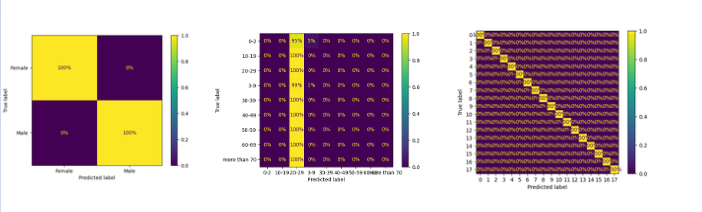
\includegraphics{graphics/cm_rfc.png}
    \caption[Confusion Matrix voor Random Forest Classifier]{Confusion Matrix voor Random Forest Classifier}
    \label{fig:cmrfc}}
\end{figure}

\subsection{XGBoost Classifier} \label{sub:poc-xgb}
Het XGBoost, Extreme Gradient Boosting, Classifier model wordt beschikbaar gesteld via \textit{xgboost}. Ook aan dit model kan geen tekstuele data worden meegeven en worden de labels omgezet in numerische waarden, zoals in ~\ref{sub:poc-rfc}. \\
\\
Voor de classificatie van beide labels met de MultiOutputClassifier vindt nog een preprocessing stap plaats. De tekstuele labels moeten omgezet worden naar numerische categorieën. Hiervoor wordt de LabelEncoder van \textit{sklearn.preprocessing} gebruikt. De labels worden dan samengevoegd met \textit{$np.column\_stack$}. Codevoorbeeld ~\ref{sc:prepmulti} geeft weer hoe de labels worden aangepast voor de MultiOuputClassifier. Het label voor een vrouwelijke 0-2 jarige wordt zo [0,1]. \\
\\
Aan de Grid Search voor de XGBoost Classifier worden volgende parameters meegegeven: 
\begin{itemsize}
    \item $n\_estimators$: het aantal bomen dat gebruikt wordt (default = 100). 
    \item $max\_depth$: de maximale diepte van een boom (default = 6). 
\end{itemsize}

\begin{lstlisting}[style=mystyle, caption={Functie om labels aan te passen voor de MultiOutputClassifier \autocite{Roepke2024} en \autocite{Numpy2024}}, label={sc:prepmulti}]
        age_class_encoded = label_encoder.fit_transform(y_train_age)
        gender_encoded = label_encoder.fit_transform(y_train_gender)
        y_combined = np.column_stack((age_class_encoded, gender_encoded))
    \end{lstlisting}

\begin{center}
    \begin{tabular}{||c | c | c | c||} 
        \hline
        & Geslacht & Leeftijd & Beide  \\ 
        \hline
        Parameters & $n\_estimators=267$, $depth$=5 &  $n\_estimators$=300, $depth$=4 & $n\_estimators$=100 \\ 
        \hline
        Accuracy & 94.76\% & 81,82\% & 10,23\%  \\
        \hline
        Precision & 95.22\% & 90,98\% & 6,50\%  \\
        \hline
        Recall & 94.09\% & 84,16\% & 5,35\% \\
        \hline
        Specificity & 95.41\% & 97,30\% & 94,32\% \\
        \hline
        F1 & 94.65\% & 87,44\% & 5,87\%  \\
      
    \end{tabular}
\end{center}
\\
\\
Figuur ~\ref{fig:cmxgb} geeft de confusion matrices voor de XGBoost classifier modellen weer. Hieruit kunnen we afleiden dat de XGBoost Classifier zeer goed presteert voor de aparte voorspelling van leeftijd en geslacht. Wanneer beide labels gelijktijdig worden voorspeld, presteert het model zeer slecht. Ook dit kan te verklaren zijn door overfitting, de aard van de data of het model kan geen patronen vinden. 

\begin{figure}[H]
    \centering
    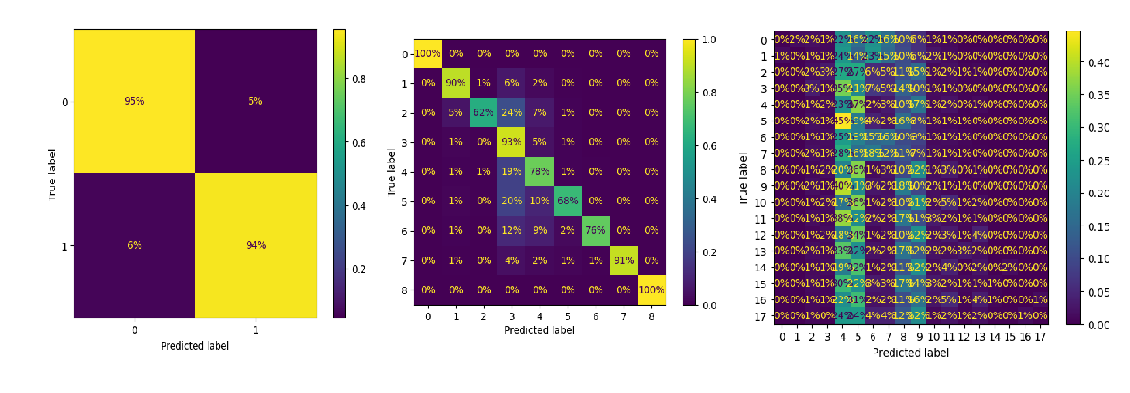
\includegraphics[width=\columnwidth]{graphics/cm_xgb.png}
    \caption[Confusion Matrix voor XGBoost Classifier]{Confusion Matrix voor XGBoost Classifier}
    \label{fig:cmxgb}}
\end{figure}
\subsection{Support Vector Machines} \label{sub:poc-svm}
Het Support Vector Classifier (SVC) model wordt beschikbaar gesteld via \textit{sklearn.svm}. Een SVM kan wel classificeren op basis van tekstuele data. Aan dit model wordt wel de originele dataset meegegeven en worden de labels niet gewijzigd. \\
\\
Aan de Grid Search voor het SVC model worden volgende parameters meegegeven:
\begin{itemize}
    \item C: regularisatie parameter, afhankelijk van de grootte van de dataset (default = 1.0).
    \item gamma: coëfficiënt van de kernel (default = 'scale')
    \item kernel: kernel type die gebruikt wordt in het algoritme (default = 'rbf').
    \item degree: graad van de kernel (default = 3).
\end{itemize}
\begin{center}
    \begin{tabular}{||c | c | c | c||} 
        \hline
        & Geslacht & Leeftijd & Beide  \\ 
        \hline
        Parameters & C=125 &  C=125, kernel='linear', degree=1 & C=25  \\ 
        \hline
        Score model (train) & 68.41\% & 21.52\% & 20.50\%  \\
        \hline
        Accuracy & 66.79\% & 28.23\% & 21.55\%  \\
        \hline
        Precision & 67.57\% & 22.12\% & 19.44\%  \\
        \hline
        Recall & 66.40\% & 21.70\% & 13.87\%  \\
        \hline
        Specificity & 67.19\% & 90.17\% & 95.15\% \\
        \hline
        F1 & 66.98\% & 21.91\% & 16.18\%  \\
       
    \end{tabular}
\end{center}
\\
\\
Figuur ~\ref{fig:svc} geeft de confusion matrices voor de SVC modellen weer. Uit de scores kan afgeleid worden dat het SVC model slechter presteert dan voorgaande modellen. Voor de voorspelling van geslacht wordt hier slechts een score van circa 70\% behaald. Ook de modellen voor de voorspelling van leeftijd en beide presteren slecht, met een score van slechts 20\%. Ook uit de confusion matrices is af te leiden dat er veel foute voorspellingen zijn. Hieruit kan geconcludeerd worden dat een SVC niet het geschikte model is voor de classificatie van gezichtsafbeeldingen. 
\\
\begin{figure}[H]
    \centering
    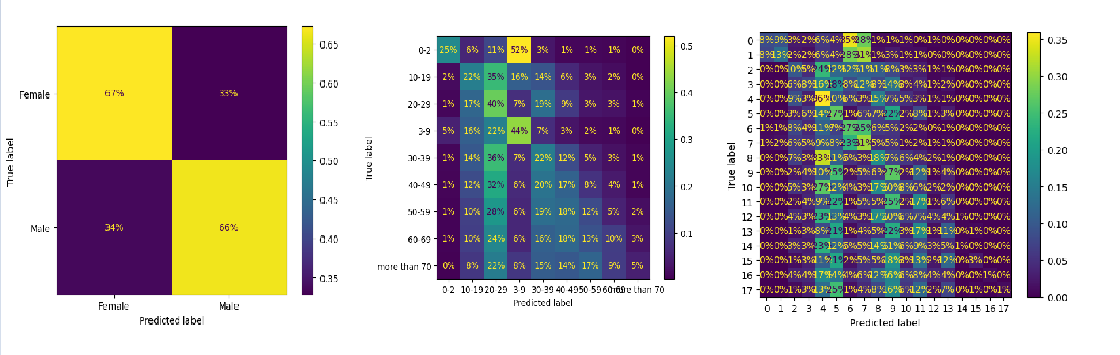
\includegraphics[width=\columnwidth]{graphics/cm_svc.png}
    \caption[Confusion Matrix voor Support Vector Classifier]{Confusion Matrix voor Support Vector Classifier}
    \label{fig:svc}}
\end{figure}
\subsection{Voting Classifier} \label{sub:poc-votingclass}
De Voting Classifier is een ensemble techniek die meerdere modellen combineert. De SVC, random forest en XGBoost Classifier worden tegelijk aangesproken om de accuracy van het model te verhogen. De parameters die het beste scoorden voor de afzonderlijke modellen worden hier hergebruikt. Codevoorbeeld ~\ref{?} geeft weer hoe de Voting Classifier de verschillende modellen combineert. 

\begin{center}
    \begin{tabular}{||c c c c||} 
        \hline
        & Geslacht & Leeftijd & Beide  \\ 
        \hline
        Parameters & ? &  ? & ?  \\
        \hline
        Accuracy & ?\% & ?\% & ?\%  \\
        \hline
        Precision & ?\% & ?\% & ?\%  \\
        \hline
        Recall & ?\% & ?\% & ?\%  \\
        \hline
        Specificity & ?\% & ?\% & ?\% \\
        \hline
        F1 & ?\% & ?\% & ?\%  \\
        
    \end{tabular}
\end{center}